\documentclass[UTF8]{beamer}
\usepackage{graphicx, color}
\usepackage{algorithm2e}
\usepackage{zhspacing}
\usepackage{amsmath}

\usepackage{underscore}
\usetheme{JuanLesPins}
\usepackage{fontspec}
\setsansfont{Microsoft YaHei}

\usepackage{enumerate}

\AtBeginSection[]{
  \frame{
    \frametitle{Next}
    \tableofcontents[currentsection, subsectionstyle=show/shaded/hide]
  }
}

\AtBeginSubsection[]{
  \frame{
    \frametitle{Next}
    \tableofcontents[currentsubsection]
  }
}

\title{Introduction to Perl}

\author{Gang Chen\\ chengang@bgitechsolutions.com}

\logo{
\includegraphics[width=1.3cm]{bgi-logo.png}
\includegraphics[width=2.5cm]{cuhklogo.png}}
\date{\today}




\begin{document}


\begin{frame}
\titlepage
\end{frame}
\begin{frame}[t]\frametitle{Outline}
\tableofcontents[hideallsubsections]
\end{frame}

\section{Overview}

\begin{frame}[t]{What is Perl?}
\begin{block}{Perl}
  \begin{itemize}
    \item Practical Extraction and Report Language
    \item Pathologically Eclectic Rubbish Lister
  \end{itemize}
\end{block}
\end{frame}
%--- Next Frame ---%

\begin{frame}[t]{Perl: History 1}
\begin{columns}
  \begin{column}{.7\textwidth}
\begin{itemize}
  \item 1.0: December 18, 1987, Larry Page
  \item 2.0: 1988, a better regular expression
  \item 3.0: 1989, support binary data streams
  \item 4.0, 1991
  \item Programming Perl, Camel Book, for Perl 4.0
\end{itemize}
\end{column}
\begin{column}{.3\textwidth}
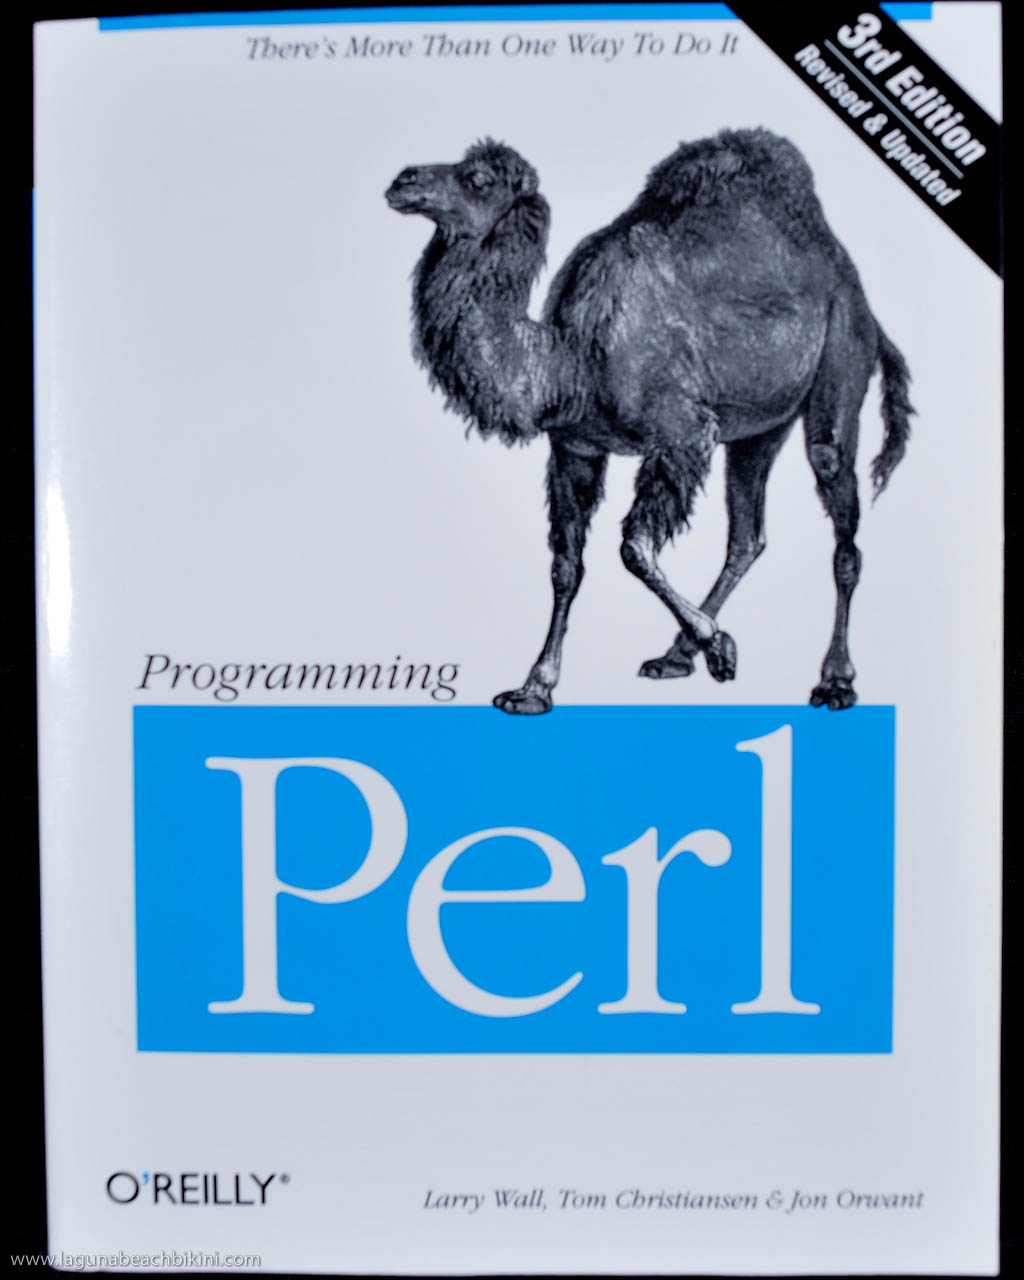
\includegraphics[width=\textwidth]{programmingperl.jpg}
\end{column}
\end{columns}
\end{frame}
%--- Next Frame ---%

\begin{frame}[t]{Perl: History 2}
\begin{block}{Perl 5}
  \begin{itemize}
    \item 5.000: October 17, 1994, rewrite of the interpreter\\
    Objects, lexical variables, modules and references are added.
    \item 5.002: new prototypes feature.
    \item Comprehensive Perl Archive Network(CPAN), 1995.
    \item 5.004: May 15, 1997, UNIVERSAL package and CGI.pm module.
    \item 5.8: July 18, 2002, unicode, a new I/O, thread
    \item 5.10: December 18, 2007
    \item 5.20: May 27, 2014, subroutin signature, slice.
  \end{itemize}
\end{block}
\end{frame}
%--- Next Frame ---%

\begin{frame}[t]{Perl: History 3}
\begin{block}{Perl 6}
  \begin{itemize}
    \item Perl 6 design process was first announced on July 19, 2000
    \item As of 2014, none of Perl 6 implementation are considered ``complete''.
    \begin{itemize}
      \item Rakudo Perl: Perl 6 for virtual machines.
      \item Pugs: Perl 6 written in Haskell.
      \item v6.pm: a pure Perl 5 implementation of Perl 6.
      \item Yapsi: a Perl 6 compiler and runtime written in Perl 6 itself.
    \end{itemize}
  \end{itemize}
\end{block}
\end{frame}
%--- Next Frame ---%

\begin{frame}[t]{Applications}
\begin{block}{Applications}
  \begin{itemize}
    \item text processing
    \item CGI programming: Craigslist, IMDb, Slashdot and so on;
    \item graphics programming: Perl/Tk, WxPerl
    \item system administration
    \item network programming
    \item bioinformatics
  \end{itemize}
\end{block}
\end{frame}
%--- Next Frame ---%

\begin{frame}[t]{References}
\begin{block}{Books}
  \begin{itemize}
    \item Learning Perl sixth Edition;
    \item Mastering Perl;
    \item Advanced Perl;
    \item Programming Perl;
  \end{itemize}
\end{block}
\begin{block}{Official Website}
  http://www.perl.org/
\end{block}
\end{frame}
%--- Next Frame ---%

\section{Quick Get Started}

\begin{frame}[t]{Install}
\begin{block}{Download and Install}
  Download: http://www.perl.org/get.html
  \begin{itemize}
    \item Unix/Linux: preinstalled
    \item Mac OS: preinstalled
    \item Windows:
    \begin{itemize}
      \item ActiveState Perl: A binary distribution for Win
      \item StrawBerry Perl: Open source
      \item DWIM Perl: based on StrawBerry and include many useful CPAN modules
    \end{itemize}
  \end{itemize}
\end{block}
\end{frame}
%--- Next Frame ---%

\begin{frame}[t]{Install: editor}
\begin{block}{Editors}
  \begin{itemize}
    \item Vim: editor god
    \item Emacs: god's editor
    \item Notepad++: fast and easy to use
    \item Atom, sublime text, textmate \ldots
  \end{itemize}
\end{block}
\end{frame}
%--- Next Frame ---%


\begin{frame}[t]{Hello Perl!}
  \centerline{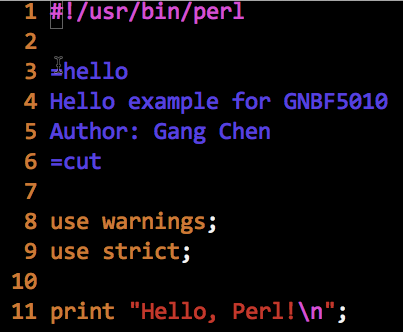
\includegraphics[height=.6\textheight]{hello.png}}
  see hello.pl
\end{frame}
%--- Next Frame ---%

\begin{frame}[t]{Input and Run}
  \begin{enumerate}
    \item Input the source codes by using a editor
    \item Save the source codes to a file named hello.pl
    \item Execute the file:
    \begin{itemize}
      \item Add execution permission to the file and execute directly
      \item Execute the file by using perl interpreter
    \end{itemize}
  \end{enumerate}
\end{frame}
%--- Next Frame ---%

\section{Syntax}

\subsection{Basic Syntax}
\begin{frame}[fragile]{Scalar Data: Number}
\begin{verbatim}
  $a = 1;
  $b = 1.2;
  print $a + $b, "\n";
\end{verbatim}
\end{frame}
%--- Next Frame ---%

\begin{frame}[t]{Scalar Data: String}
  \centerline{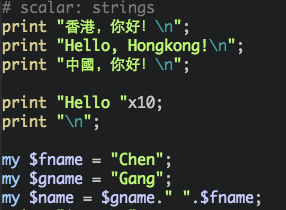
\includegraphics[height=.6\textheight]{string.png}}
\end{frame}
%--- Next Frame ---%

\begin{frame}[fragile]{Conversion between Numbers and Strings}
\begin{verbatim}
  # conversion between numbers and strings
  print 1 + 2, "\n";
  print "1" + 2, "\n";
  print "1" + "2", "\n";
  print "1 + 2", "\n";

  print "00001" + "002", "\n";

  print "one" + 2, "\n";
  print "one" + "two", "\n";
\end{verbatim}
\end{frame}
%--- Next Frame ---%

\begin{frame}[fragile]{if Control Structure}
\begin{verbatim}
  # if control structure
  my $num1 = 5;
  my $num2 = 3;

  if($num1 > $num2){
    print "Success\n";
  }else{
    print "failed\n";
  }

  $num1 > $num2 ? print "Success\n" : print "Failed\n";

  print "Success\n" if ($num1 > $num2);
\end{verbatim}
\end{frame}
%--- Next Frame ---%

\begin{frame}[fragile]{while and for}
\begin{verbatim}
# while and for
my $num = 1;
while($num < 10){
  print $num, "\n";
  $num++;
}

for($num = 1;$num<10;$num++){
  print $num, "\n";
}
\end{verbatim}
\end{frame}
%--- Next Frame ---%

\begin{frame}[t]{List and Array}
\begin{block}{List and Array}
  \begin{description}
    \item[List] A list is an ordered collection of scalars.
    \item[Array] An array is a variable that contains a list.
  \end{description}
\end{block}
\centerline{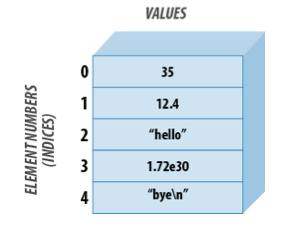
\includegraphics[height=.4\textheight]{list.png}}
\end{frame}
%--- Next Frame ---%

\begin{frame}[fragile]{List and Array}
\begin{verbatim}
  # list and array
  my @list1 = (1,2,3,4,5);
  my @list2 = ("one", "two", "three");
  my @list3 = (1..10);
  print $list1[0], "\n";
  print $list2[1], "\n";
  print $list3[3], "\n";
\end{verbatim}
\end{frame}
%--- Next Frame ---%

\begin{frame}[fragile]{List and Array}
\begin{itemize}
  \item Operate to the start of the array: shift, unshift
  \item Operate to the end of the array: pop, push
  \item Any place: splice
\end{itemize}
\end{frame}
%--- Next Frame ---%

\begin{frame}[fragile]{foreach}
\begin{verbatim}
  foreach (@list1){
    print $_, "\n";
  }

  for(@list1){
    print $_, "\n";
  }

  print $_, "\n" for(@list1);

  print $_, "\n" for(1..10);
\end{verbatim}
\end{frame}
%--- Next Frame ---%

\begin{frame}[t]{Hash}
  \centerline{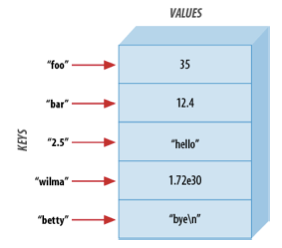
\includegraphics[height=.6\textheight]{hash.png}}
\end{frame}
%--- Next Frame ---%

\begin{frame}[fragile]{Hash}
\begin{verbatim}
  # hash
  my %scores = (
    'Gang' => 60,
    'Chen' => 70,
    'Xu' => 80,
    'Lu' => 90,
  );

  print $scores{'Chen'}, "\n";

  for (keys %scores){
    print $_,":",$scores{$_},"\n";
  }

  print $_,":",$scores{$_},"\n" for (keys %scores);

  print $_, "\n" for(values %scores);
\end{verbatim}
\end{frame}
%--- Next Frame ---%

\subsection{Input and Output}

\begin{frame}[fragile]{Input from User}
\begin{verbatim}
  print "What's your name?\n";

  my $name = <STDIN>;
  print "Hello ", $name;

  my @names = <STDIN>;

  print "Hello ", $_ for(@names);
\end{verbatim}
\end{frame}
%--- Next Frame ---%

\begin{frame}[fragile]{Interact with Filesystem}
  see io.pl
\end{frame}
%--- Next Frame ---%

\subsection{Regular Expression}

\begin{frame}[t]{Regular Expression}
\begin{block}{Regular Expression}
  Regular Expression is a template or pattern of strings.
\end{block}
\end{frame}
%--- Next Frame ---%

\begin{frame}[t]{Match}
  see regex.pl
\end{frame}
%--- Next Frame ---%

\begin{frame}[t]{References}
  \begin{itemize}
    \item Mastering Regular Expressions
    \item 精通正则表达式
    \item 正则指引
  \end{itemize}
\end{frame}
%--- Next Frame ---%


\section{Examples}

\subsection{System Administration}

\begin{frame}[fragile]{Command Options of perl}
\begin{block}{Options}
  \begin{itemize}
    \item -e
    \item -n
    \begin{verbatim}
while (<>) {
  # your code goes here
}
    \end{verbatim}
    \item -p
\begin{verbatim}
  while (<>) {
      # your code goes here
    } continue {
      print or die "-p destination: $!\n";
    }
\end{verbatim}
  \end{itemize}
\end{block}
\end{frame}
%--- Next Frame ---%

\begin{frame}[fragile]{Process file content}
\begin{block}{Adding Line Number to file content}
  \begin{verbatim}
    perl -ne 'print "$. $_"' names.txt
    perl -pe '$_ = "$. $_"' names.txt
  \end{verbatim}
\end{block}
\end{frame}
%--- Next Frame ---%

\subsection{CGI Programming}

\begin{frame}
  \centerline{\Huge{Thanks!}}
\end{frame}
%--- Next Frame ---%

\end{document}
